\documentclass[portrait,final,a0paper,fontscale=0.277]{baposter}

\usepackage{calc}
\usepackage{graphicx}
\usepackage{amsmath}
\usepackage{amssymb}
\usepackage{relsize}
\usepackage{multirow}
\usepackage{rotating}
\usepackage{bm}
\usepackage{url}
\usepackage{xcolor}
\usepackage{enumitem}

\usepackage{graphicx}
\usepackage{multicol}

%\usepackage{times}
%\usepackage{helvet}
%\usepackage{bookman}
\usepackage{palatino}

\newcommand{\captionfont}{\footnotesize}
\setlist[itemize]{leftmargin=*}
\graphicspath{{images/}{../images/}}
\usetikzlibrary{calc}

%%%%%%%%%%%%%%%%%%%%%%%%%%%%%%%%%%%%%%%%%%%%%%%%%%%%%%%%%%%%%%%%%%%%%%%%%%%%%%%%
%%%% Some math symbols used in the text
%%%%%%%%%%%%%%%%%%%%%%%%%%%%%%%%%%%%%%%%%%%%%%%%%%%%%%%%%%%%%%%%%%%%%%%%%%%%%%%%

%%%%%%%%%%%%%%%%%%%%%%%%%%%%%%%%%%%%%%%%%%%%%%%%%%%%%%%%%%%%%%%%%%%%%%%%%%%%%%%%
% Multicol Settings
%%%%%%%%%%%%%%%%%%%%%%%%%%%%%%%%%%%%%%%%%%%%%%%%%%%%%%%%%%%%%%%%%%%%%%%%%%%%%%%%
\setlength{\columnsep}{1.5em}
\setlength{\columnseprule}{0mm}

%%%%%%%%%%%%%%%%%%%%%%%%%%%%%%%%%%%%%%%%%%%%%%%%%%%%%%%%%%%%%%%%%%%%%%%%%%%%%%%%
% Save space in lists. Use this after the opening of the list
%%%%%%%%%%%%%%%%%%%%%%%%%%%%%%%%%%%%%%%%%%%%%%%%%%%%%%%%%%%%%%%%%%%%%%%%%%%%%%%%
\newcommand{\compresslist}{%
\setlength{\itemsep}{1pt}%
\setlength{\parskip}{0pt}%
\setlength{\parsep}{0pt}%
}

\begin{document}

% Define some colors
\definecolor{lightblue}{rgb}{1, 1, 1}
\definecolor{darkblue}{rgb}{0,0.1294,0.2784}

\hyphenation{resolution occlusions effects assessing non-additive inattentiveness phenotype liability restricted developed studies detecting structure confound evolution selection recombination prohibitive computationally epitopes decreases account}

\begin{poster}%
  % Poster Options
  {
  % Show grid to help with alignment
  grid=false,
  % Column spacing
  colspacing=0.7em,
  % Color style
  bgColorOne=white,
  bgColorTwo=white,
  borderColor=darkblue,
  headerColorOne=darkblue,
  headerColorTwo=lightblue,
  headerFontColor=white,
  boxColorOne=white,
  boxColorTwo=darkblue,
  % Format of textbox
  textborder=roundedsmall,
  % Format of text header
  eyecatcher=false,
  headerborder=closed,
  headerheight=0.12\textheight,
%  textfont=\sc, An example of changing the text font
  headershape=smallrounded,
  headershade=shadelr,
  headerfont=\Large\bf\textsc, %Sans Serif
  textfont={\setlength{\parindent}{1.5em}},
  boxshade=plain,
%  background=shade-tb,
  background=plain,
  linewidth=2pt
  }
  % Eye Catcher - Weird - have to include.
  {\includegraphics[height=5em]{images/graph_occluded.pdf}} 
  % Title
  {\vspace{0.3em}\bf Mapping the drivers of within-host \\ pathogen evolution using massive data
sets\vspace{0.2em}}
  % Authors
  % {{\bf D. S. Palmer} [1,2,3]; A. Bloemendal [1,2]; B. M. Neale [1,2,3]; N. Patterson [1,4]\\
  {\small{{\bf DS Palmer} [1]; I Turner [1]; S Fidler [2]; J Frater [1]; D Goedhals [3]; P Goulder [1,4]; KH Huang [1];\\
  A Oxenius [5]; R Phillips [1]; R Shapiro [6,7]; C Van Vuuren [3]; AR McLean [1] and G McVean [1].}\\
 \smaller{1) University of Oxford, Oxford. 2) Imperial College, London. 3) University of KwaZulu-Natal, Durban. 4) University of the Free State, Bloemfontein.\\
 5) Swiss Federal Institute of Technology, Zurich. 6) Botswana Harvard AIDS Institute Partnership, Gaborone. 7) Harvard School of Public Health, Boston.}
  }
  % University logos
  {% The makebox allows the title to flow into the logo, this is a hack because of the L shaped logo.
    
\includegraphics[width=0.18\textwidth]{images/oxford.pdf}\\
  }
%%%%%%%%%%%%%%%%%%%%%%%%%%%%%%%%%%%%%%%%%%%%%%%%%%%%%%%%%%%%%%%%%%%%%%%%%%%%%%
%%% Now define the boxes that make up the poster
%%%---------------------------------------------------------------------------
%%% Each box has a name and can be placed absolutely or relatively.
%%% The only inconvenience is that you can only specify a relative position 
%%% towards an already declared box. So if you have a box attached to the 
%%% bottom, one to the top and a third one which should be in between, you 
%%% have to specify the top and bottom boxes before you specify the middle 
%%% box.
%%%%%%%%%%%%%%%%%%%%%%%%%%%%%%%%%%%%%%%%%%%%%%%%%%%%%%%%%%%%%%%%%%%%%%%%%%%%%%

%%%%%%%%%%%%%%%%%%%%%%%%%%%%%%%%%%%%%%%%%%%%%%%%%%%%%%%%%%%%%%%%%%%%%%%%%%%%%%
\headerbox{Motivations}{name=introduction,column=0,row=0,span=1}{
\noindent Differences among hosts can impact within-host pathogen evolution.\vspace{5pt}

\noindent Identifying such interactions can be achieved through genetic association studies.\vspace{5pt}

\noindent However, extensive genetic population structure in hosts and pathogens can confound analyses.\vspace{5pt}

% \noindent Moreover, the multiple testing burden of interaction scanning can potentially limit power.\vspace{5pt}

\noindent Phylogenetic methods that help to account for confounding are computationally prohibitive and do not account for recombination.
}
\headerbox{Conclusions}{name=conclusions,column=1,span=2,above=bottom}{
\noindent We have developed a Bayesian approach for detecting host influences on pathogen evolution that makes use of vast existing data sets of pathogen diversity to improve power and control for stratification.

\noindent We recover well known CTL escape mutants in HIV, observe strong overlap between curated lists of epitopes and those identified here, and detect novel associations.
}
%%%%%%%%%%%%%%%%%%%%%%%%%%%%%%%%%%%%%%%%%%%%%%%%%%%%%%%%%%%%%%%%%%%%%%%%%%%%%%
\headerbox{Our Model Approximation}{name=simulations,column=1,span=2}{
%%%%%%%%%%%%%%%%%%%%%%%%%%%%%%%%%%%%%%%%%%%%%%%%%%%%%%%%%%%%%%%%%%%%%%%%%%%%%%
\hspace{-6mm}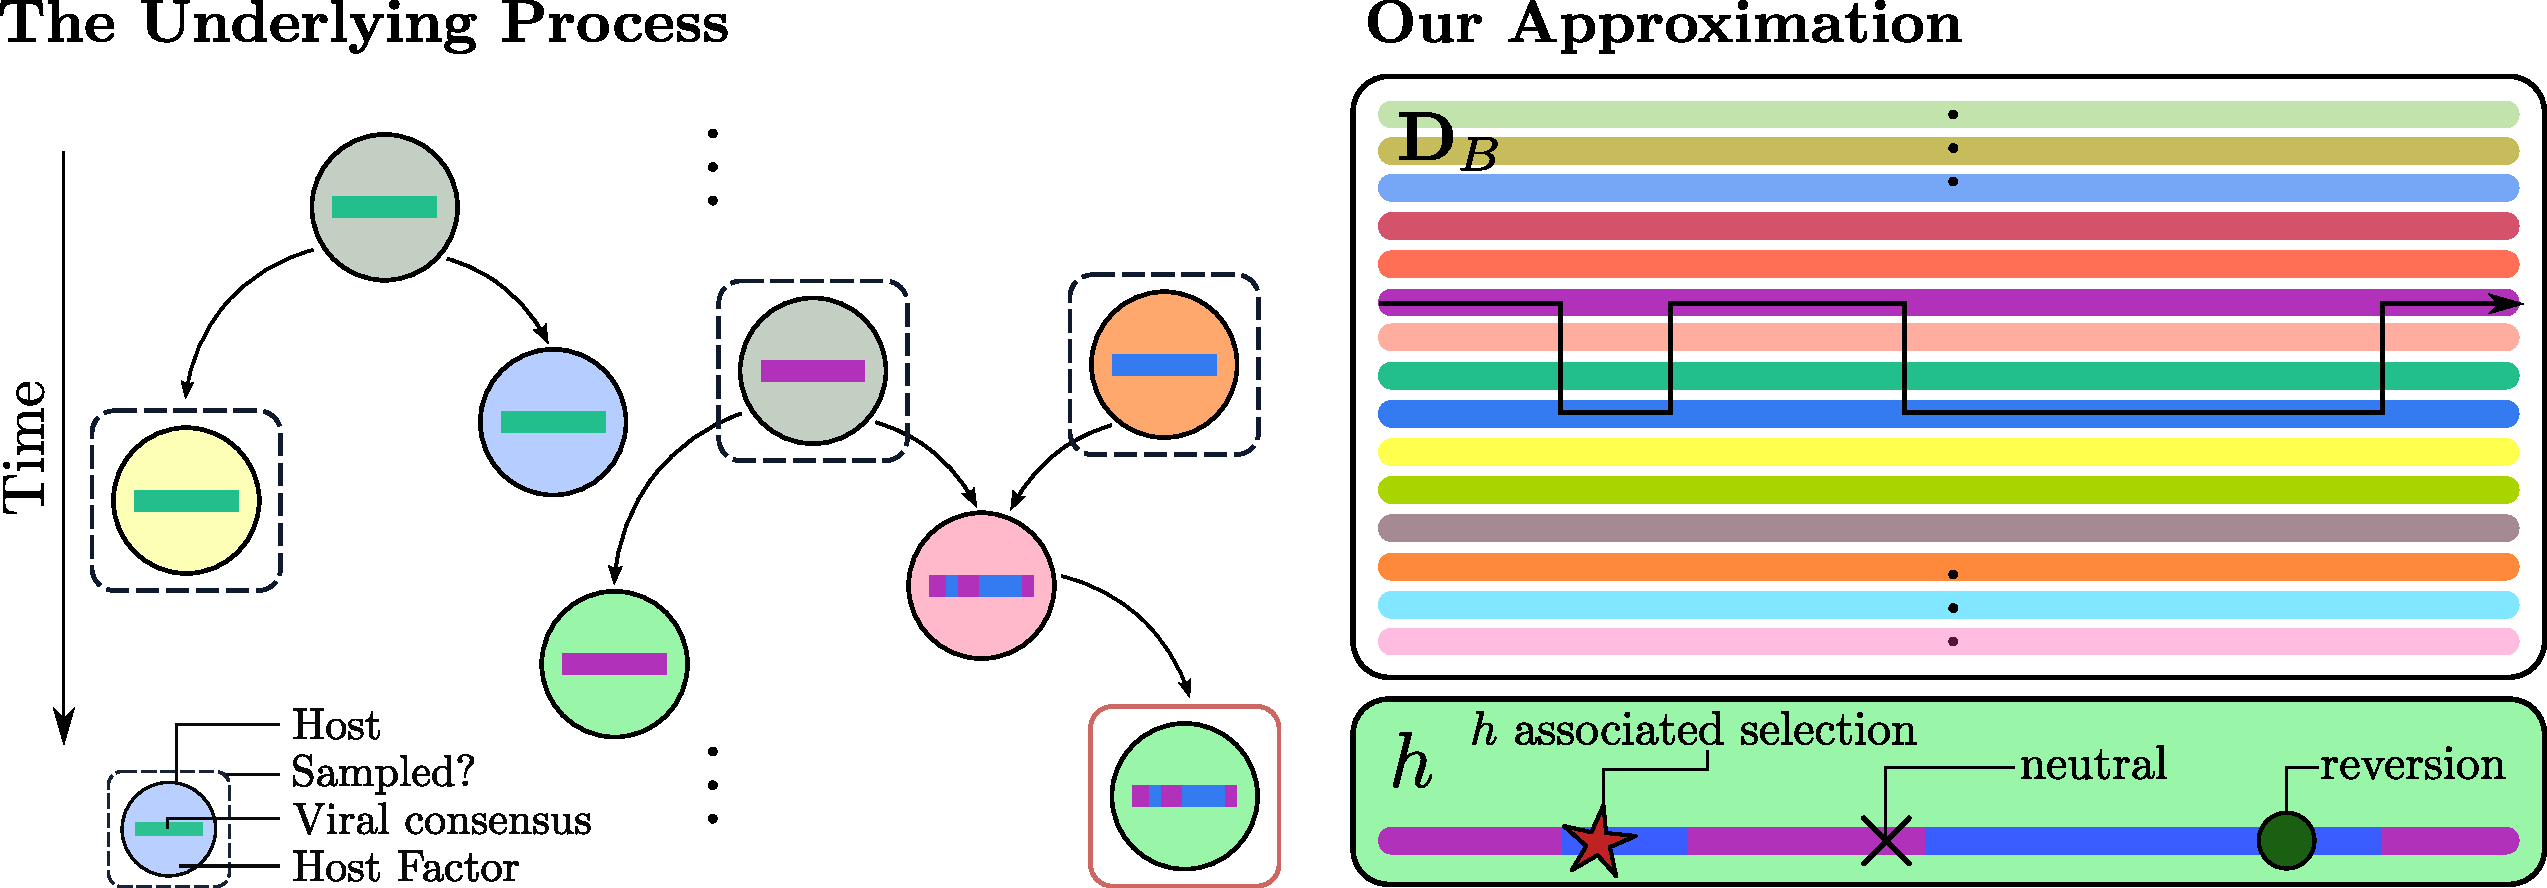
\includegraphics[width=\linewidth]{Fig1_updated.pdf}\vspace{2mm}
{\bf Our approximation}:
Pathogen sequences in $\mathbf{D}$ arise from $\mathbf{D}_B$ through recombination and mutation \cite{LiSteph}, modulated by host factors of $\mathbf{D}$ (host factor $= h$ in the cartoon).

\vspace{0.3em}
\noindent All selection along a lineage connecting each member of $\mathbf{D}$ to $\mathbf{D}_B$ occurred within the host that the member of $\mathbf{D}$ was isolated from $\Rightarrow$ only host factor information for $\mathbf{D}$ is required.

\vspace{0.3em}
\noindent Using a codon model, we model host factor associated selection at each codon as a scaling of the non-synonymous mutation rate away from the consensus viral sequence - we call this $\gamma_i^h$.
}

\headerbox{Results}{name=results,column=1,span=2,below=simulations,above=conclusions}{
\noindent We apply our approach to HIV and host HLA information, to estimate HLA associated selection along the viral genome.

\vspace{0.3em}
\noindent $\mathbf{D}_B =$ all HIV sequence data in public databases ($|\mathbf{D}_B|=148,866$ for reverse transcriptase).

\vspace{0.3em}
\noindent $\mathbf{D}=$ HIV sequence data and host HLA data in the Los Alamos HIV Database, and curated data from the UK, Switzerland, South Africa and Botswana ($|\mathbf{D}|=2,681$ for reverse transcriptase).

\vspace{0.6em}
\noindent We detect well-known HLA associated selection - e.g. in B$^*$51 restricted $\mathtt{TAFTIPSI}$.

\vspace{0.6em}
\hspace{-4mm}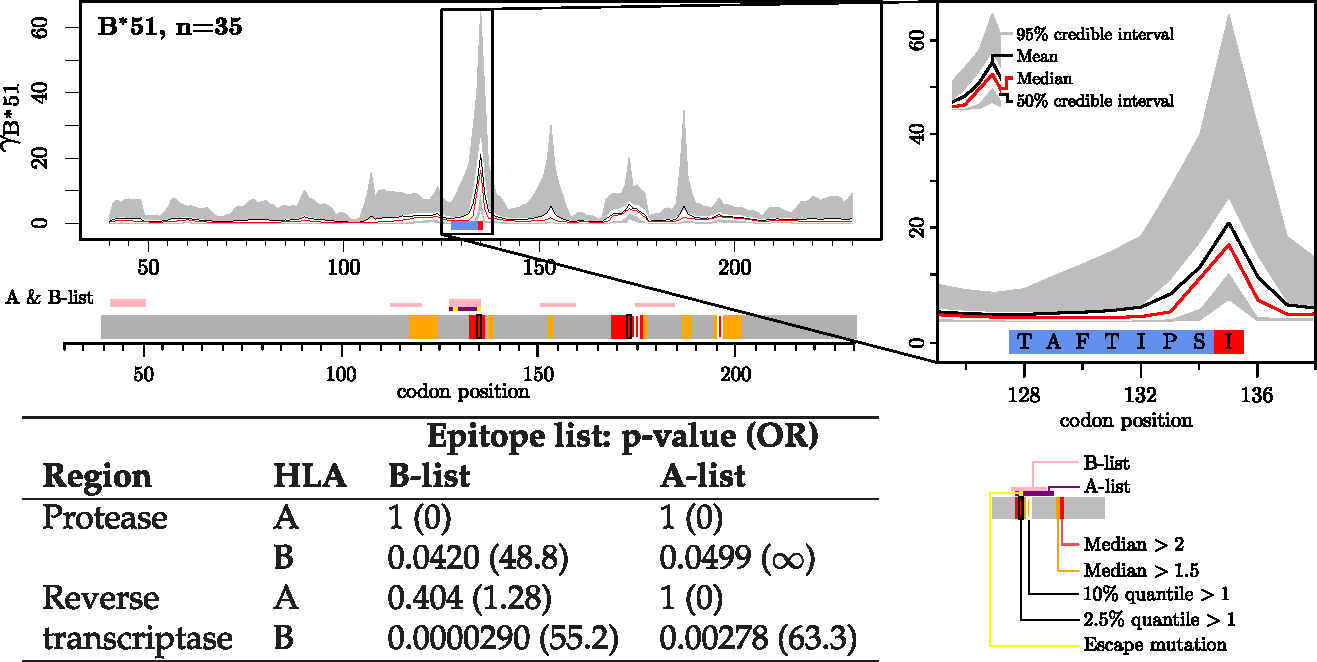
\includegraphics[width=0.98\linewidth]{Fig4_new.pdf}

\vspace{0.6em}
\noindent {\bf Compare to previous work on epitope restriction}\vspace{-2mm}
\begin{itemize}
\item Our strong candidate sites: median $\gamma_i^h$ > 2, 2.5\% quantile > 1.\vspace{-2mm}
\item classify documented epitopes
\begin{itemize}\vspace{-2mm}
\item A-list = best-defined experimentally determined HIV epitopes.\vspace{-1mm}
\item B-list = all HIV epitopes reported in the literature.
\end{itemize}
\end{itemize}
% \begin{center}
% \begin{tabular}{lllll}\hline
% &&\multicolumn{2}{c}{{\bf Epitope list: p-value (OR)}}\\
% {\bf Region}                & {\bf HLA} & {\bf B-list}          & {\bf A-list}            \\ \hline
% Protease              & A       & 1 (0)            & 1 (0)             \\
%                       % &     & 0.0855     & 0.160 (4.12)     & 0.166 (9.00)      \\
%                       & B            & 0.0420 (48.8)    & 0.0499 ($\infty$) \\  
%                       % &     & 0.964      & 0.213 (3.50)     & 0.0335 (14.0)     \\ 
% Reverse               & A        & 0.404 (1.28)     & 1 (0)             \\
%                       % &     & 0.935      & 0.122 (1.57)     & 0.499 (1.61)      \\
% transcriptase         & B         & 0.0000290 (55.2) & 0.00278 (63.3)    \\
%                             % & 0.303      & 0.000250 (19.4)  & 0.00278 (37.7)    \\
% \hline
% \end{tabular}
% \end{center}
\noindent Permuting labellings of HLAs, we find strong evidence for enrichment of selection at A-list epitopes for HLA-B. As confidence in the epitope collection or the strength of selection decreases, so does the enrichment.  
%%%%%%%%%%%%%%%%%%%%%%%%%%%%%%%%%%%%%%%%%%%%%%%%%%%%%%%%%%%%%%%%%%%%%%%%%%%%%%
}
%%%%%%%%%%%%%%%%%%%%%%%%%%%%%%%%%%%%%%%%%%%%%%%%%%%%%%%%%%%%%%%%%%%%%%%%%%%%%%
% \headerbox{Future Work}{name=futurework,column=2,span=1,below=results,above=bottom}{
%%%%%%%%%%%%%%%%%%%%%%%%%%%%%%%%%%%%%%%%%%%%%%%%%%%%%%%%%%%%%%%%%%%%%%%%%%%%%%
% \noindent Apply to other `measurably evolving' pathogens, e.g. Hepatitis C.
% }
%%%%%%%%%%%%%%%%%%%%%%%%%%%%%%%%%%%%%%%%%%%%%%%%%%%%%%%%%%%%%%%%%%%%%%%%%%%%%%
% \headerbox{Our Approach}{name=method,column=0,below=introduction}{
% }
\headerbox{Simulations}{name=sims,column=0,below=introduction}{
\noindent We repeat the following $100$ times:
\begin{itemize}
\item Simulate a pathogen genealogy using a birth death process ($1,000,000$ extant leaves).
\item Lay down mutations using a codon model of host factor associated selection, choosing a set of sites under strong host factor associated selection.
\item Subsample $\mathbf{D}$ and $\mathbf{D}_B$ at the leaves\\($|\mathbf{D}_B|=100,000$, $|\mathbf{D}|=460$).
\item Determine strength of host factor associated selection at each codon/amino acid for each host factor.
\end{itemize}
We can then create ROC curves for different methods in the literature.

\vspace{1em}
\hspace{-5mm}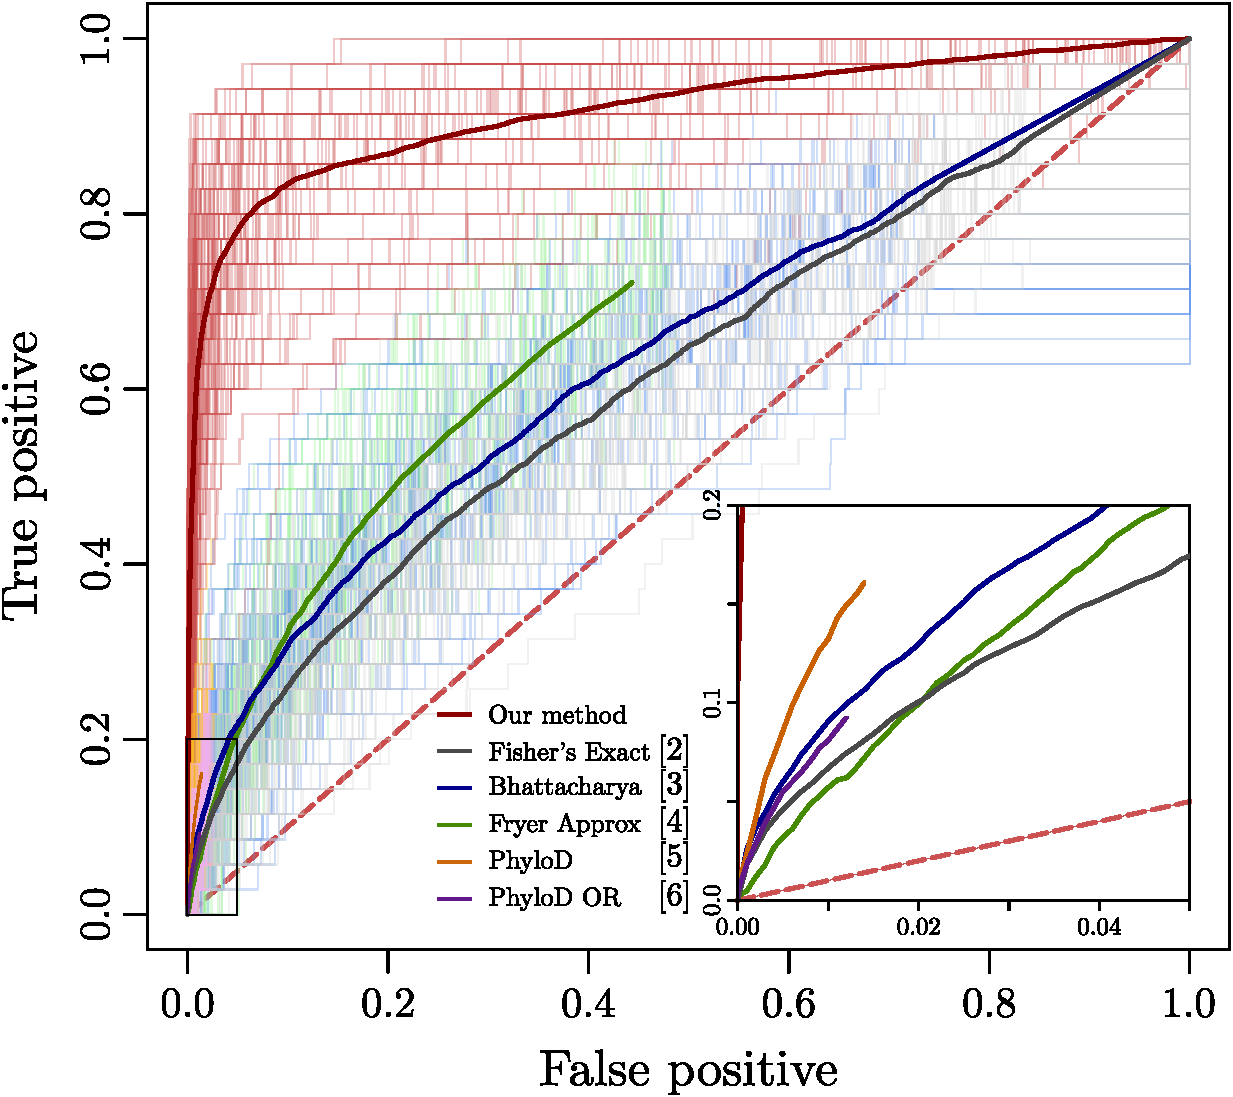
\includegraphics[width=\linewidth]{Fig2.pdf}
Making use of $\mathbf{D}_B$ drastically increases our power.
}

%%%%%%%%%%%%%%%%%%%%%%%%%%%%%%%%%%%%%%%%%%%%%%%%%%%%%%%%%%%%%%%%%%%%%%%%%%%%%%
\headerbox{References}{name=references,column=0,span=1,above=bottom,below=sims}{
% \begin{multicols}{2}
%%%%%%%%%%%%%%%%%%%%%%%%%%%%%%%%%%%%%%%%%%%%%%%%%%%%%%%%%%%%%%%%%%%%%%%%%%%%%%
\footnotesize
    \bibliographystyle{ieee}
    \renewcommand{\section}[2]{\vskip 0.05em}
      \begin{thebibliography}{1}\itemsep=-0.01em
      \setlength{\baselineskip}{0.4em}
      \bibitem{LiSteph}
        Li and Stephens, 2003. \emph{Genetics.}
      \bibitem{LDscore1}
        Moore \emph{et al.}, 2002. \emph{Science.}
      \bibitem{Swedes}
        Bhattacharya \emph{et al.}, 2007. \emph{Science.}
      \bibitem{Helen}
      Fryer \emph{et al.}, 2010. \emph{PLoS Pathogens.}
      \bibitem{Carlson1}
        Carlson \emph{et al.}, 2008. \emph{PLoS Computational Biology.}
      \bibitem{Carlson2}
        Carlson \emph{et al.}, 2012. \emph{Journal of Virology.}
        \bibitem{LLano}
        Llano \emph{et al.}, 2013. \emph{hiv.lanl.gov.}
      \end{thebibliography}
  % \noindent
  % Source code is available at \\
  % \url{http://www.github.com/astheeggeggs/mcqueen}
  % \end{multicols}
  \vspace{3mm}
  \includegraphics[width=\linewidth]{QR_code.pdf}
  }

%%%%%%%%%%%%%%%%%%%%%%%%%%%%%%%%%%%%%%%%%%%%%%%%%%%%%%%%%%%%%%%%%%%%%%%%%%%%%%


\end{poster}

\end{document}

